\documentclass[12pt]{article}
\usepackage[margin=1in]{geometry}
\usepackage{graphicx}
\usepackage{booktabs}
\usepackage{caption}
\usepackage{setspace}
\usepackage{float}
\usepackage{hyperref}
\usepackage{amsmath}

\setstretch{1.2}
\title{Problem Set 5 \\ \large{Education Spending and Student Outcomes}}
\author{Ayse Deniz}
\date{October 2025}

\begin{document}
\maketitle

\begin{abstract}
This problem set examines the relationship between per-student education spending and 8th grade math achievement using state-year panel data. 
Descriptive visualizations illustrate key trends across states, while econometric models quantify the association through baseline OLS and fixed-effects specifications. 
All figures and regression tables are generated directly from the accompanying Python analysis scripts to ensure full reproducibility.
\end{abstract}

\section*{Research Question}
How is per-student education spending related to student achievement in the United States?  
Secondary questions include:  
\begin{itemize}
  \item Does the relationship between education spending and achievement change when accounting for state and year effects?  
  \item To what extent do differences across states drive the observed correlation between spending and test scores?  
\end{itemize}

\section{Data and Summary}
The raw dataset was preprocessed in Python to remove incomplete observations and create key analytical variables. 
The dataset used is \texttt{states\_all\_extended.csv}, obtained from Kaggle’s public dataset repository. 
It contains state-level data on education finances and student performance compiled from the U.S. Department of Education’s National Center for Education Statistics (NCES). 
The data include revenues, expenditures, and NAEP 8th-grade math scores for U.S. states from 2000 to 2015. 
The main cleaning and construction steps are summarized below:

\begin{itemize}
  \item Dropped rows with missing values for enrollment, instructional expenditure, or 8th grade math scores.
  \item Computed \texttt{spend\_per\_student} = \texttt{INSTRUCTION\_EXPENDITURE} / \texttt{ENROLL}.
  \item Created the main explanatory variable \texttt{log\_spending} = $\log(\texttt{spend\_per\_student})$.
  \item Standardized state names (uppercase and underscores) and set the panel index as (\texttt{STATE}, \texttt{YEAR}).
  \item Saved cleaned data for use in generating visuals and estimating panel models.
\end{itemize}

After cleaning and constructing the key variables, the resulting dataset contains the following variables used in the analysis:

\begin{itemize}
  \item \textbf{8th Grade Math Score (NAEP):} outcome variable measuring average state-level achievement.
  \item \textbf{Instruction Spending per Student:} instruction expenditure divided by total student enrollment.
  \item \textbf{Log of Instruction Spending per Student:} logarithmic transformation of per-student spending, used as the main explanatory variable.
\end{itemize}

\section{Descriptive Visualizations}
\begin{figure}[H]
  \centering
  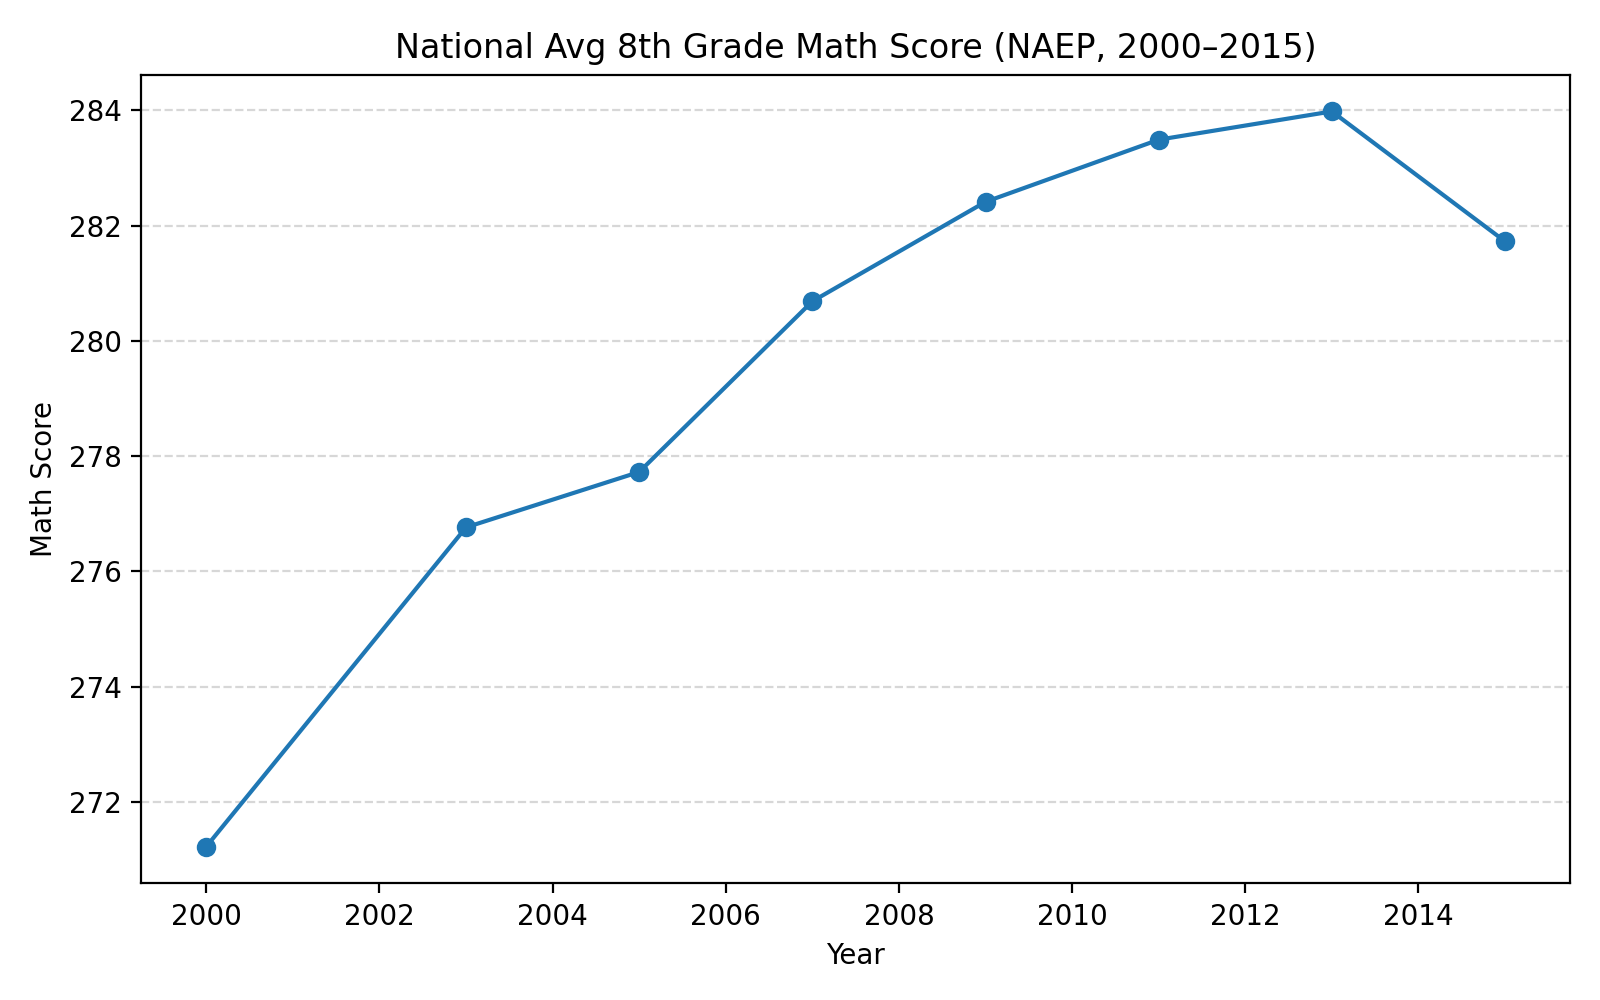
\includegraphics[width=0.85\textwidth]{images/fig1_math_trend.png}
  \caption{National average 8th grade math score (by year).}
  \label{fig:math_trend}
\end{figure}

\begin{figure}[H]
  \centering
  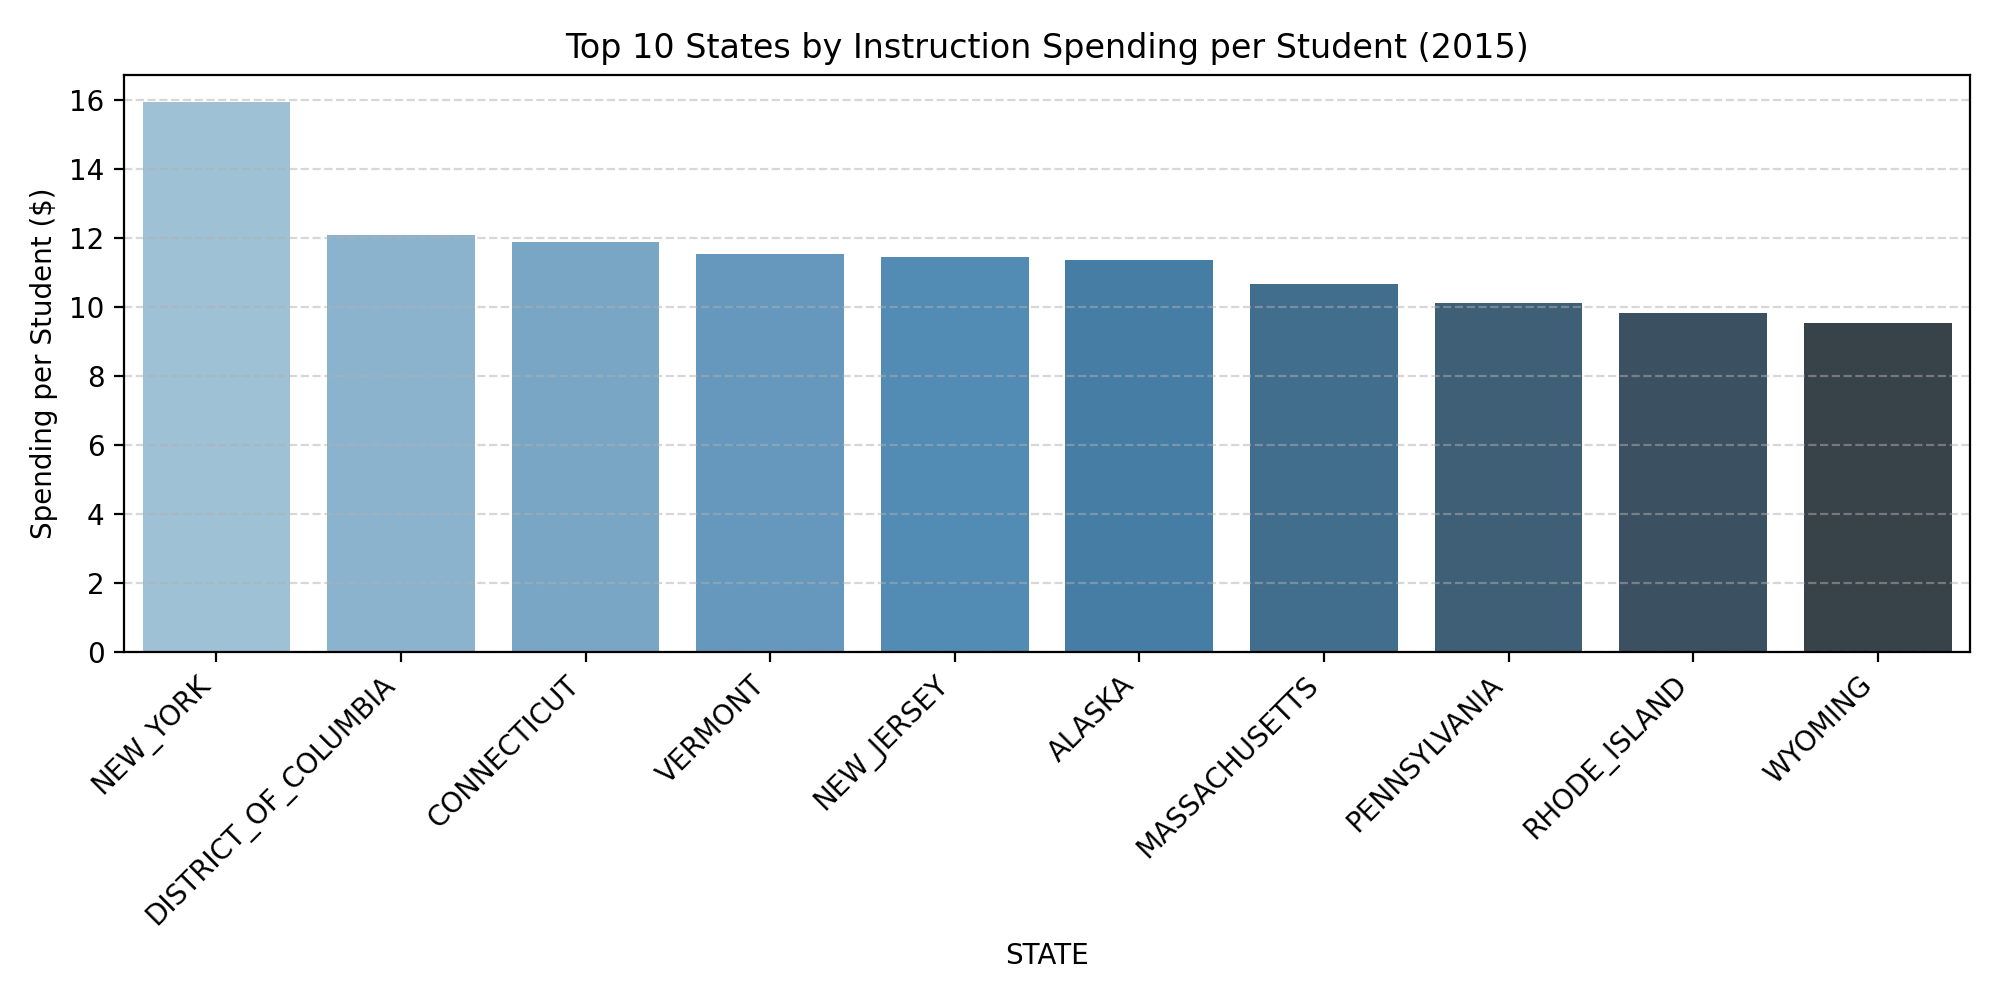
\includegraphics[width=0.85\textwidth]{images/fig2_top_spending_states.png}
  \caption{Top 10 states by instruction spending per student (latest year in the sample).}
  \label{fig:top_states}
\end{figure}

\begin{figure}[H]
  \centering
  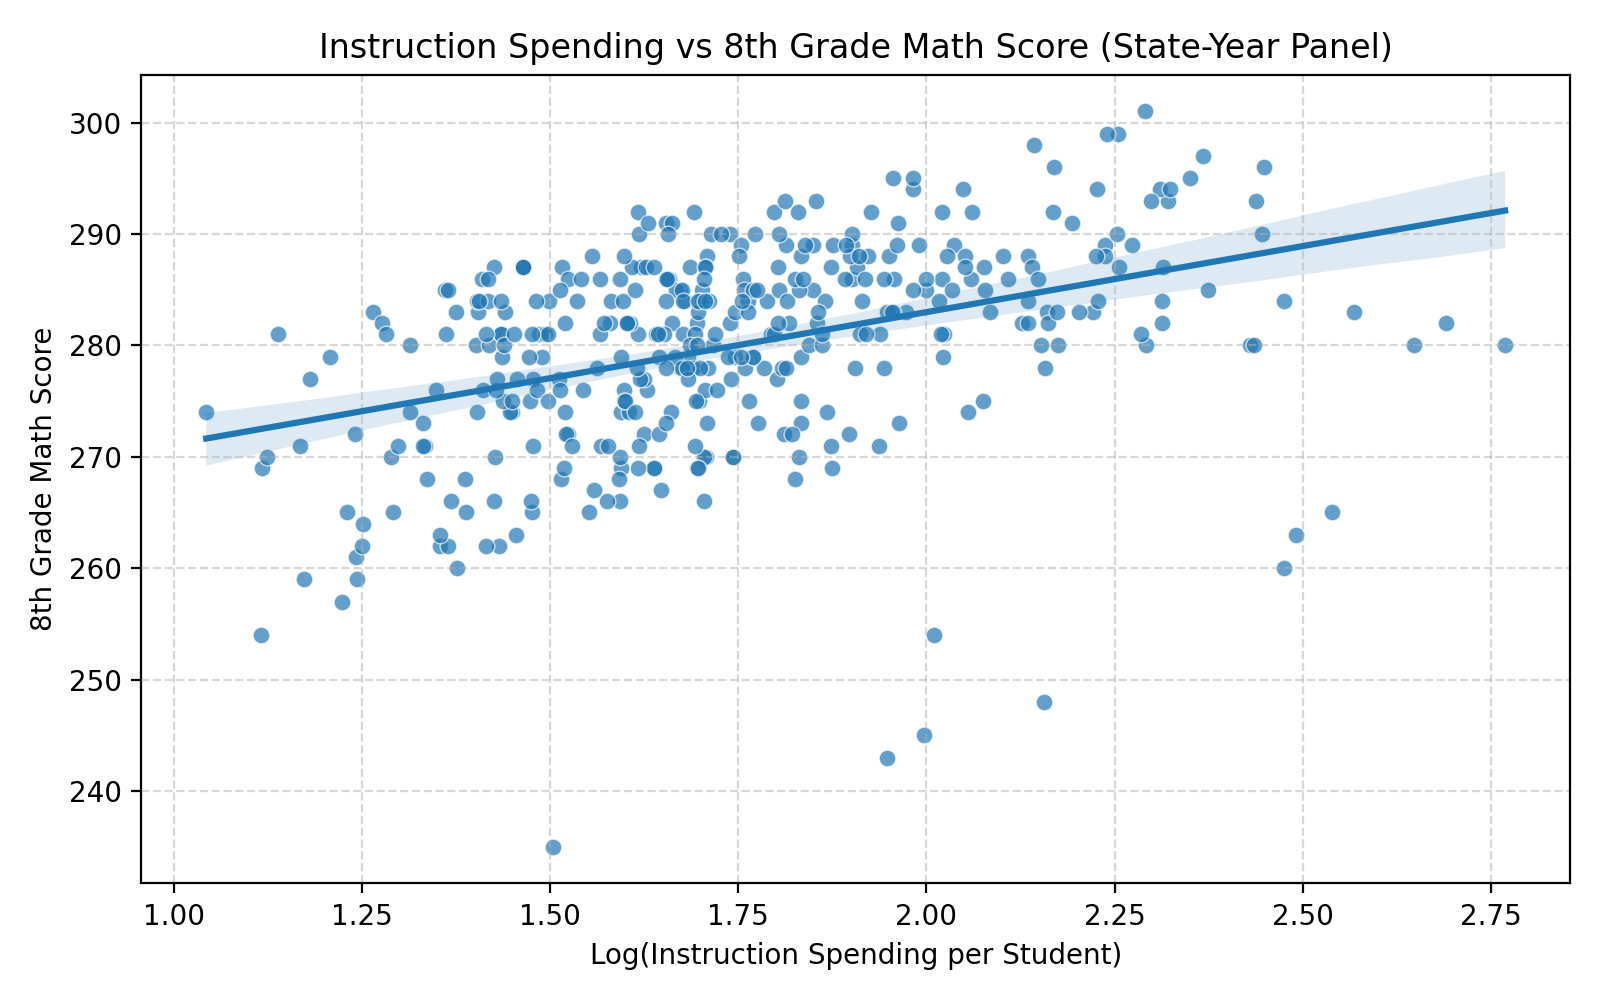
\includegraphics[width=0.85\textwidth]{images/fig3_spending_vs_score.png}
  \caption{Scatter of log spending per student vs. 8th grade math score (state-year panel).}
  \label{fig:spending_vs_score}
\end{figure}

\section{Econometric Models and Results}
We estimate three models (all estimated in \texttt{ps5\_models.py} and written to \texttt{results.tex}):
\begin{enumerate}
  \item \textbf{Baseline OLS:} $Math_{it} = \alpha + \beta \log(\text{spend}_{it}) + \varepsilon_{it}$
  \item \textbf{State fixed effects:} controls for unobserved, time-invariant differences across states.
  \item \textbf{Two-way fixed effects:} includes both state and year effects, controlling for state heterogeneity and national time shocks.
\end{enumerate}

\begin{center}
% Auto-generated regression summary

\begin{tabular}{lrrr}
\toprule
Model & Log Spending & Std. Error & R-squared \\
\midrule
Baseline OLS & 11.86 & 1.65 & 0.16 \\
State FE & 19.03 & 1.56 & 0.62 \\
Two-Way FE & 5.86 & 5.37 & 0.03 \\
\bottomrule
\end{tabular}

\vspace{0.3em}

\vspace{0.3em}
\end{center}

\section*{Interpretation}
The regression results highlight the relationship between instructional spending and student achievement across U.S. states. 
The coefficient on log spending is positive in all models, indicating that higher per-student instructional spending is associated with higher average 8th grade math scores.

\begin{itemize}
  \item \textbf{Baseline OLS:} The coefficient on log spending reflects the unconditional correlation between spending and test scores. States that spend more tend to have higher achievement levels on average.
  \item \textbf{State Fixed Effects:} Controlling for time-invariant state characteristics (e.g., policy environment, persistent demographics) strengthens the relationship, suggesting that within-state increases in spending are linked to higher test performance.
  \item \textbf{Two-Way Fixed Effects:} Adding year fixed effects accounts for national shocks and trends over time. The coefficient decreases in magnitude, implying that part of the observed OLS association was driven by persistent differences across states rather than short-run causal effects.
\end{itemize}

Overall, these models provide evidence of a positive association between education spending and student achievement, though they do not establish causality. Further research could explore causal identification using policy changes or funding reforms as natural experiments.

\section*{Appendix: Reproducibility Test}
The full analysis pipeline was executed using the provided Bash script (\texttt{run\_ps5.sh}). 
All unit tests passed successfully, and the final \texttt{ProblemSet5\_Ayse.pdf} was automatically generated. 

\begin{figure}[h!]
  \centering
  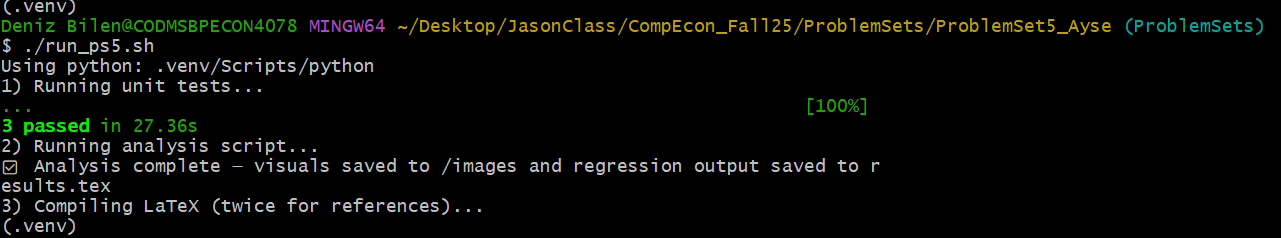
\includegraphics[width=\textwidth]{Screenshot_ps5.png}
  \caption{Terminal output showing successful execution of the reproducible pipeline.}
  \label{fig:pytest_output}
\end{figure}

\section*{Conclusion}
This analysis provides evidence of a positive association between education spending and 8th grade math achievement. 
While higher per-student spending is correlated with better test outcomes, this relationship should not be interpreted as causal. 
Identifying a causal effect would require policy variation or experimental settings that isolate exogenous changes in school funding.

\end{document}
